\scanpage{15}\mspage{14}
% ink top, relations
Si on se donne à la fois les deux relations
\[
\left\{\begin{aligned}
\unsure{\underline R|R}(a,b)&\qquad \{a,b\}\in\mathrm{Drap}_2(\mathcal L)\\
R(a,b,c)&\qquad b\text{ est str. entre }a\text{ et }c
\end{aligned}\right.
\]
alors pour récupérer le biordre, il suffit de supposer $\mathcal L$ filtrant croissant et filtrant décroissant, \deleted{et les relations \unsure{Si|si}, \unsure{Cet|cet|Oct} \unsure{sur les}, filtrant \unsure{cr.} et \unsure{décr.} \unsure{sont} de \unsure{qque|toutes} \unsure{comp.|faç.} \unsure{connexes|connues en} \unsure{$S_0$|$v_0$|$0$}} 

% ink middle, On va voir
\deleted{\unsure{On va}} On va voir maintenant comment la connaissance\inserted{ de $\mathrm{Drap}_2(\mathcal L)$, et} pour $\unsure{\varepsilon|\mathcal E|E}\in\mathrm{Drap}_2(\deleted{\unsure{I}}\mathcal L)$, de la décomp. de
% ink middle, C(\unsure{\varepsilon|\mathcal E|E}) and continuation
\[
 C(\unsure{\varepsilon|\mathcal E|E})=\{\,t\in\mathcal L\deleted{\unsure{\notin\varepsilon|\smallsetminus\varepsilon}}\mid
 \deleted{\unsure{x}}\{\unsure{\varepsilon|\mathcal E|E}\unsure{\cup|,}t\}\deleted{\unsure{=|-}}\in\mathrm{Drap}_3(\mathcal L)\,\}
\]
en composantes connexes, implique la connaissance de la relation
\[
 R(a,b,c)\unsure{\mathord{:}|\mathord{?}}\quad b\text{ strict entre }a\text{ et }c.
\]
% ink lower third, Première condition
Première condition : $\{a,b,c\}\in\mathrm{Drap}_3(\mathcal L)$ (résulte de la donnée de $\mathrm{Drap}_2(\mathcal L)$)
\figure{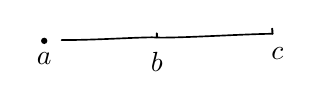
\begin{tikzpicture}[x=1cm,y=1cm,line cap=round]
\fill (0,0) circle (1.15pt);
\draw[line width=.6pt] (.22,.01) .. controls (.66,.01) and (1.06,.04) .. (1.37,.045) .. controls (1.61,.026) and (2.48,.085) .. (2.9,.09);
\draw[line width=.7pt] (1.43,.045) -- (1.43,.095) (2.9,.09) -- (2.895,.155);
\node[below] at (0,-.025) {$a$};
\node[below] at (1.43,-.015) {$b$};
\node[below] at (2.96,.035) {$c$};
\end{tikzpicture}}
% ink bottom, final sentence and cancelled display
Si $b$ est entre $a$ et $c$, regardons les
\[
 \deleted{J_{abc}=\text{composante de }C(\{a,b\}}\unsure{,|)}
\]

% pale vertical watermark
\rotatebox{90}{\textsc{\unsure{ng Extra Stro}}}
